\documentclass[journal,12pt,twocolumn]{IEEEtran}
%
\usepackage{setspace}
\usepackage{gensymb}
\usepackage{xcolor}
%\usepackage{esint}
\usepackage{caption}
%\usepackage{subcaption}
%\doublespacing
\singlespacing
\usepackage{multicol}

\usepackage{iithtlc}
%\usepackage{graphicx}
%\usepackage{amssymb}
%\usepackage{relsize}
\usepackage[cmex10]{amsmath}
\usepackage{mathtools}
%\usepackage{amsthm}
%\interdisplaylinepenalty=2500
%\savesymbol{iint}
%\usepackage{txfonts}
%\restoresymbol{TXF}{iint}
%\usepackage{wasysym}
\usepackage{amsthm}
\usepackage{mathrsfs}
\usepackage{txfonts}
\usepackage{stfloats}
\usepackage{cite}
\usepackage{cases}
\usepackage{subfig}
%\usepackage{xtab}
\usepackage{longtable}
\usepackage{multirow}
%\usepackage{algorithm}
%\usepackage{algpseudocode}
\usepackage{enumitem}
\usepackage{mathtools}
%\usepackage{stmaryrd}

\usepackage{listings}
%    \usepackage[latin]{inputenc}                                 %%
    \usepackage{color}                                            %%
    \usepackage{array}                                            %%
    \usepackage{longtable}                                        %%
    \usepackage{calc}                                             %%
    \usepackage{multirow}                                         %%
    \usepackage{hhline}                                           %%
    \usepackage{ifthen}                                           %%
  %optionally (for landscape tables embedded in another document): %%
    \usepackage{lscape}   
    \usepackage{tikz}
\usetikzlibrary{calc}
\usepackage{tkz-euclide}
\usetkzobj{all}
  
%\usepackage{tikz}
%\usepackage{tkz-euclide}
%\usetkzobj{all}
%%\usepackage[utf8]{inputenc}
%\usepackage{rotating}
%\usetikzlibrary{arrows,shapes,decorations.markings,positioning}
%\usepackage{amsmath}
%\usepackage{ulem}
%\usepackage{soul}

%\usepackage{wasysym}
%\newcounter{MYtempeqncnt}
\DeclareMathOperator*{\Res}{Res}
%\renewcommand{\baselinestretch}{2}
\renewcommand\thesection{\arabic{section}}
\renewcommand\thesubsection{\thesection.\arabic{subsection}}
\renewcommand\thesubsubsection{\thesubsection.\arabic{subsubsection}}

\renewcommand\thesectiondis{\arabic{section}}
\renewcommand\thesubsectiondis{\thesectiondis.\arabic{subsection}}
\renewcommand\thesubsubsectiondis{\thesubsectiondis.\arabic{subsubsection}}

%\DeclareUnicodeCharacter{01B5}{\zst}
%\DeclareRobustCommand\zst{%
%\unskip\nobreak\thinspace\zbar\allowbreak\thinspace\ignorespaces}
%\newcommand{\zbar}{\raisebox{0.2ex}{--}\kern-0.6em Z}


% correct bad hyphenation here
\hyphenation{op-tical net-works semi-conduc-tor}

\def\inputGnumericTable{}  

\lstset{
language=python,
frame=single, 
breaklines=true
}

\begin{document}
%

\theoremstyle{definition}
\newtheorem{theorem}{Theorem}[section]
\newtheorem{problem}{Problem}
\newtheorem{proposition}{Proposition}[section]
\newtheorem{lemma}{Lemma}[section]
\newtheorem{corollary}[theorem]{Corollary}
\newtheorem{example}{Example}[section]
\newtheorem{definition}{Definition}[section]
%\newtheorem{algorithm}{Algorithm}[section]
%\newtheorem{cor}{Corollary}
\newcommand{\BEQA}{\begin{eqnarray}}
\newcommand{\EEQA}{\end{eqnarray}}
\newcommand{\define}{\stackrel{\triangle}{=}}

\bibliographystyle{IEEEtran}
%\bibliographystyle{ieeetr}



\providecommand{\pr}[1]{\ensuremath{\Pr\left(#1\right)}}
\providecommand{\qfunc}[1]{\ensuremath{Q\left(#1\right)}}
\providecommand{\sbrak}[1]{\ensuremath{{}\left[#1\right]}}
\providecommand{\lsbrak}[1]{\ensuremath{{}\left[#1\right.}}
\providecommand{\rsbrak}[1]{\ensuremath{{}\left.#1\right]}}
\providecommand{\brak}[1]{\ensuremath{\left(#1\right)}}
\providecommand{\lbrak}[1]{\ensuremath{\left(#1\right.}}
\providecommand{\rbrak}[1]{\ensuremath{\left.#1\right)}}
\providecommand{\cbrak}[1]{\ensuremath{\left\{#1\right\}}}
\providecommand{\lcbrak}[1]{\ensuremath{\left\{#1\right.}}
\providecommand{\rcbrak}[1]{\ensuremath{\left.#1\right\}}}
\theoremstyle{remark}
\newtheorem{rem}{Remark}
\newcommand{\sgn}{\mathop{\mathrm{sgn}}}
\providecommand{\abs}[1]{\left\vert#1\right\vert}
\providecommand{\res}[1]{\Res\displaylimits_{#1}} 
\providecommand{\norm}[1]{\lVert#1\rVert}
\providecommand{\mtx}[1]{\mathbf{#1}}
\providecommand{\mean}[1]{E\left[ #1 \right]}
\providecommand{\fourier}{\overset{\mathcal{F}}{ \rightleftharpoons}}
%\providecommand{\hilbert}{\overset{\mathcal{H}}{ \rightleftharpoons}}
\providecommand{\system}{\overset{\mathcal{H}}{ \longleftrightarrow}}
\providecommand{\gauss}[2]{\mathcal{N}\ensuremath{\left(#1,#2\right)}}
	%\newcommand{\solution}[2]{\textbf{Solution:}{#1}}
\newcommand{\solution}{\noindent \textbf{Solution: }}
\providecommand{\dec}[2]{\ensuremath{\overset{#1}{\underset{#2}{\gtrless}}}}
%\numberwithin{equation}{section}
%\numberwithin{problem}{section}
\makeatletter
\@addtoreset{figure}{problem}
\makeatother

\let\StandardTheFigure\thefigure
%\renewcommand{\thefigure}{\theproblem.\arabic{figure}}
\renewcommand{\thefigure}{\theproblem}

\def\putbox#1#2#3{\makebox[0in][l]{\makebox[#1][l]{}\raisebox{\baselineskip}[0in][0in]{\raisebox{#2}[0in][0in]{#3}}}}
     \def\rightbox#1{\makebox[0in][r]{#1}}
     \def\centbox#1{\makebox[0in]{#1}}
     \def\topbox#1{\raisebox{-\baselineskip}[0in][0in]{#1}}
     \def\midbox#1{\raisebox{-0.5\baselineskip}[0in][0in]{#1}}


% paper title
% can use linebreaks \\ within to get better formatting as desired
\title{
\logo{
Complex Analysis in Electrical Engineering
}
}
%
%
% author names and IEEE memberships
% note positions of commas and nonbreaking spaces ( ~ ) LaTeX will not break
% a structure at a ~ so this keeps an author's name from being broken across
% two lines.
% use \thanks{} to gain access to the first footnote area
% a separate \thanks must be used for each paragraph as LaTeX2e's \thanks
% was not built to handle multiple paragraphs
%

%\author{Y Aditya, A Rathnakar and G V V Sharma$^{*}$% <-this % stops a space
\author{G V V Sharma$^{*}$% <-this % stops a space
\thanks{*The author is with the Department
of Electrical Engineering, Indian Institute of Technology, Hyderabad
502205 India e-mail:  gadepall@iith.ac.in.All content in this manual is released under GNU GPL.  Free and open source.}% <-this % stops a space
%\thanks{J. Doe and J. Doe are with Anonymous University.}% <-this % stops a space
%\thanks{Manuscript received April 19, 2005; revised January 11, 2007.}}
}
% note the % following the last \IEEEmembership and also \thanks - 
% these prevent an unwanted space from occurring between the last author name
% and the end of the author line. i.e., if you had this:
% 
% \author{....lastname \thanks{...} \thanks{...} }
%                     ^------------^------------^----Do not want these spaces!
%
% a space would be appended to the last name and could cause every name on that
% line to be shifted left slightly. This is one of those "LaTeX things". For
% instance, "\textbf{A} \textbf{B}" will typeset as "A B" not "AB". To get
% "AB" then you have to do: "\textbf{A}\textbf{B}"
% \thanks is no different in this regard, so shield the last } of each \thanks
% that ends a line with a % and do not let a space in before the next \thanks.
% Spaces after \IEEEmembership other than the last one are OK (and needed) as
% you are supposed to have spaces between the names. For what it is worth,
% this is a minor point as most people would not even notice if the said evil
% space somehow managed to creep in.



% The paper headers
%\markboth{Journal of \LaTeX\ Class Files,~Vol.~6, No.~1, January~2007}%
%{Shell \MakeLowercase{\textit{et al.}}: Bare Demo of IEEEtran.cls for Journals}
% The only time the second header will appear is for the odd numbered pages
% after the title page when using the twoside option.
% 
% *** Note that you probably will NOT want to include the author's ***
% *** name in the headers of peer review papers.                   ***
% You can use \ifCLASSOPTIONpeerreview for conditional compilation here if
% you desire.




% If you want to put a publisher's ID mark on the page you can do it like
% this:
%\IEEEpubid{0000--0000/00\$00.00~\copyright~2007 IEEE}
% Remember, if you use this you must call \IEEEpubidadjcol in the second
% column for its text to clear the IEEEpubid mark.



% make the title area
\maketitle

%\tableofcontents

\begin{abstract}
This manual provides applications of Complex Analysis in Electrical Engineering.
%
\end{abstract}
% IEEEtran.cls defaults to using nonbold math in the Abstract.
% This preserves the distinction between vectors and scalars. However,
% if the journal you are submitting to favors bold math in the abstract,
% then you can use LaTeX's standard command \boldmath at the very start
% of the abstract to achieve this. Many IEEE journals frown on math
% in the abstract anyway.

% Note that keywords are not normally used for peerreview papers.
%\begin{IEEEkeywords}
%Cooperative diversity, decode and forward, piecewise linear
%\end{IEEEkeywords}



% For peer review papers, you can put extra information on the cover
% page as needed:
% \ifCLASSOPTIONpeerreview
% \begin{center} \bfseries EDICS Category: 3-BBND \end{center}
% \fi
%
% For peerreview papers, this IEEEtran command inserts a page break and
% creates the second title. It will be ignored for other modes.
\IEEEpeerreviewmaketitle


%\newpage
%\section{Two Variable}
%
%\subsection{Multivariate Gaussian}
%
\section{The Inverse Z Transform}
\begin{problem}
Show that $z^{n}$ is analytic everywhere for $n \ge 0$.
\end{problem}
\begin{problem}
Show that for $C: z = Re^{\j\theta}, 0 < \theta < 2\pi$,
\begin{equation}
\ointctrclockwise_C \frac{dz}{z^n} =
\begin{cases}
2\pi \j & n = 1
\\ 
 0 & \text{otherwise}
\end{cases}
\end{equation}
\end{problem}
\begin{definition}
The Z transform of $x(n)$ is defined as
\begin{equation}
\label{eq:z_def}
X(z)=\sum _{k=-\infty }^{\infty }x(k)z^{-k}
\end{equation}
\end{definition}
\begin{problem}
Show that
\begin{align}
\frac{1}{2\pi\j}\ointctrclockwise_C X(z)z^{n-1}\,dz  &=\sum _{k=-\infty }^{\infty }x(k)\ointctrclockwise_C z^{n-k-1}\,dz
\\
&=x(n)
\end{align}
\end{problem}
\begin{problem}
The $Z$ transform of $x(n)$ is given by
\begin{equation}
X(z) = \frac{z^{20}}{\brak{z-\frac{1}{2}}\brak{z-2}^5\brak{z+\frac{5}{2}}^2\brak{z+3}}
\end{equation}
Also, it is known that $X(z)$ is analytic for $\abs{z} = 1$. Find $x(-18)$.
\end{problem}
\section{The Laplace Transform}
\begin{problem}
Let
\begin{equation}
\int_{-\infty}^{\infty}F(t)e^{-st}\,dt = \frac{1}{s\brak{1-s^2}} = \frac{M(s)}{s}, \quad s = \sigma + \j \omega
\end{equation}
Using the inverse fourier transform relationship, show that
\begin{equation}
\label{eq:laplace_key}
F(t)e^{-\sigma t} = \frac{1}{2\pi}\int_{-\infty}^{\infty}\frac{e^{\j\omega t}}{s\brak{1-s^2}}\,d\omega
\end{equation}
\end{problem}
%
\begin{problem}
Show that
\begin{equation}
F(t) = \frac{1}{2\pi \j}\int_{\sigma - \j \infty}^{\sigma + \j \infty}\frac{e^{s t}}{s\brak{1-s^2}}\,ds
\end{equation}
\end{problem}
\begin{problem}
Let
\begin{align}
F(t) = 
\begin{cases}
\frac{1}{2\pi \j}\ointctrclockwise_{C_1}\frac{e^{st}}{s\brak{1-s^2}}\,ds & t > 0
\\
\frac{1}{2\pi \j}\ointctrclockwise_{C_2}\frac{e^{st}}{s\brak{1-s^2}}\,ds & t < 0
\end{cases}
\end{align}
where $C_1, C_2$ are the closed contours on the left and right respectively as shown in Figs. \ref{fig:laplace_left} and \ref{fig:laplace_right}. Find $F(t)$
given that the ROC of $\frac{M(s)}{s}$ is $0 < \text{Re}\brak{s} < 1$.
\end{problem}
%
\renewcommand{\thefigure}{\theproblem.\arabic{figure}}
\begin{figure}[!h]
\centering
\resizebox {\columnwidth} {!} {
%\documentclass[journal,12pt,article]{IEEEtran}
%\usepackage{tikz}
%\usetikzlibrary{calc}
%\usepackage{tkz-euclide}
%\usetkzobj{all}
%\begin{document}



\begin{tikzpicture}
\draw (11,6) -- (11,6) arc(-100:100:-3) --cycle;
\draw (10.6,6) -- (10.6,0);
\draw (7.5,3) -- (15,3);

\draw[thick,<->] (10.6,2) -- (11,2);
\draw [thick,->](10.6,3) -- (9,5.7);

\node[below right= 1mm of {(10,6.6)}] {$j\infty$};
\node[below right= 1mm of {(9.6,0.2)}] {$-j\infty$};
\node[below left= 1mm of {(11.5,3.1)}] {$\sigma$};
\node[below left= 1mm of {(11,3.34)}] {$\times$};
\node[below left= 1mm of {(11,3)}] {$0$};
\node[below left= 1mm of {(16.5,3.3)}] {$\text{Re}(s)$};
\node[below left= 1mm of {(12.5,1.2)}] {$\text{Im}(s)$};
\node[below left= 1mm of {(9,3.34)}] {$\times$};
\node[below left= 1mm of {(9,3)}] {$-1$};
\node[below left= 1mm of {(14.5,3.34)}] {$\times$};
\node[below left= 1mm of {(14.5,3)}] {$1$};
\node[below left= 1mm of {(9.8,5.1)}] {$R\rightarrow\infty$};


\end{tikzpicture}
%\end{document}
}
\caption{}
\label{fig:laplace_left}
\end{figure}
%
\begin{figure}[!h]
\centering
\resizebox {\columnwidth} {!} {
%\documentclass[journal,12pt,article]{IEEEtran}
%\usepackage{amsmath}
%\usepackage{tikz}
%\usetikzlibrary{calc}
%\usepackage{tkz-euclide}
%\usetkzobj{all}
%\begin{document}



\begin{tikzpicture}
\draw (12,0) -- (12,0) arc(-100:100:3) --cycle;
\draw (11.5,6) -- (11.5,0);
\draw (7,3) -- (15.5,3);

\draw[thick,<->] (11.5,2) -- (12,2);
\draw [thick,->](12,3) -- (15,4.6);

\node[below right= 1mm of {(11.5,6.5)}] {$j\infty$};
\node[below right= 1mm of {(11.5,0)}] {$-j\infty$};
\node[below left= 1mm of {(12.5,3)}] {$\sigma$};
\node[below left= 1mm of {(11.9,3.34)}] {$\times$};
\node[below left= 1mm of {(11.9,3)}] {$0$};
\node[below left= 1mm of {(16.8,3.3)}] {$\text{Re}(s)$};
\node[below left= 1mm of {(11.7,0.7)}] {$I_{m}(s)$};
\node[below left= 1mm of {(9,3.34)}] {$\times$};
\node[below left= 1mm of {(9,3)}] {$-1$};
\node[below left= 1mm of {(14.5,3.34)}] {$\times$};
\node[below left= 1mm of {(14.5,3)}] {$1$};
\node[below left= 1mm of {(15.5,4.3)}] {$R\rightarrow\infty$};


\end{tikzpicture}
%\end{document}
}
\caption{}
\label{fig:laplace_right}
\end{figure}
\renewcommand{\thefigure}{\theproblem}
%\begin{figure}[!h]
%\centering
%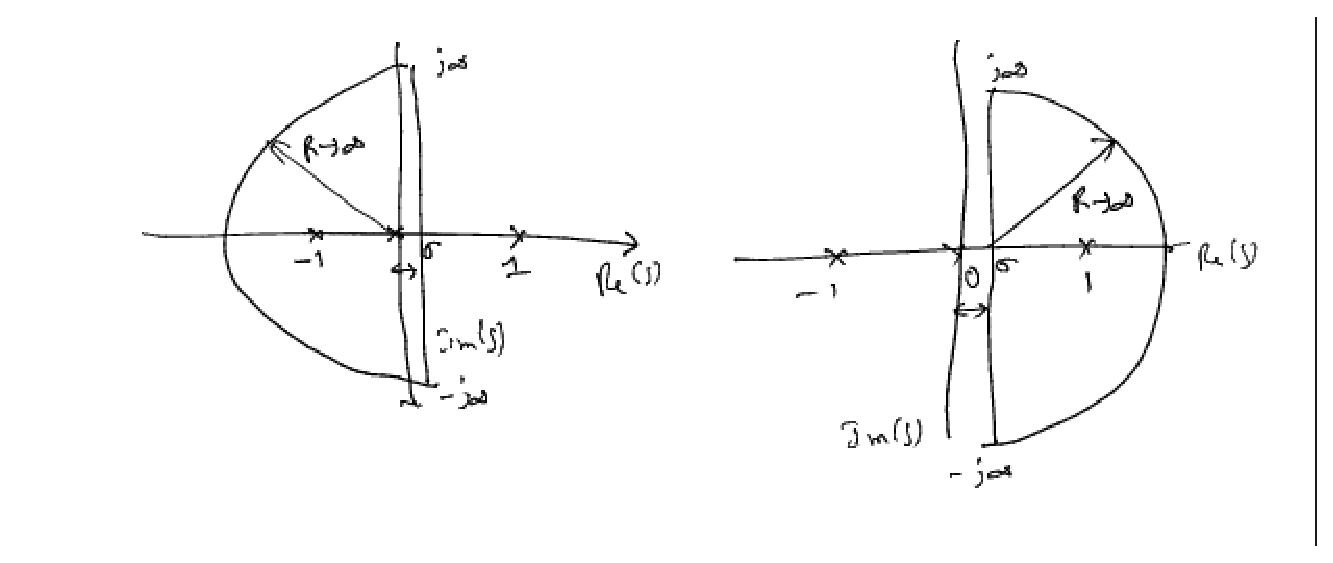
\includegraphics[width=\columnwidth]{./figs/laplace.eps}
%\caption{}
%\label{fig:laplace}
%\end{figure}
%
\section{The Gil-Pelaez Integral}
\begin{problem}
Let
\begin{equation}
\label{eq:gil}
F(t) = \frac{1}{2}-\frac{1}{2\pi\j}\times \text{c.p.v.}\int_{-\infty}^{\infty}\frac{e^{-\j\omega t}}{\omega\brak{1+\omega^2}}\,d\omega,
\end{equation}
where c.p.v. denotes the Cauchy Principal Value. Use the contour in Fig. \ref{fig:origin_contour} to evaluate $F(t), t < 0$
by showing that
\begin{enumerate}
\setlength\itemsep{0.5em}
\item
$\begin{multlined}[t]
\lim_{r\to 0}\int_{C_r}\frac{e^{-\j zt}}{z\brak{1+z^2}}\,dz = -\j\pi, 
\\
C_r: z = re^{\j\theta}, 0 < \theta < \pi
\end{multlined}$
\\
where $C_r$ is in the clockwise direction.
\item 
$\begin{multlined}[t]
\lim_{\substack{r\to 0 \\ R \to \infty}}\int_{-R}^{-r}\frac{e^{-\j\omega t}}{\omega\brak{1+\omega^2}}\,d\omega
+
\int_{r}^{R}\frac{e^{-\j\omega t}}{\omega\brak{1+\omega^2}}\,d\omega 
\\
= \j\pi + \ointctrclockwise_{C}\frac{e^{-\j zt}}{z\brak{1+z^2}}\,dz
\end{multlined}$
\end{enumerate}
\end{problem}	
%
\begin{figure}[!h]
\centering
\resizebox {\columnwidth} {!} {
%\documentclass[journal,12pt,article]{IEEEtran}
%\usepackage{tikz}
%\usepackage{amsmath}
%\usetikzlibrary{calc}
%\usepackage{tkz-euclide}
%\usetkzobj{all}
%\usetikzlibrary{arrows,shapes,decorations.markings,positioning}
%\begin{document}




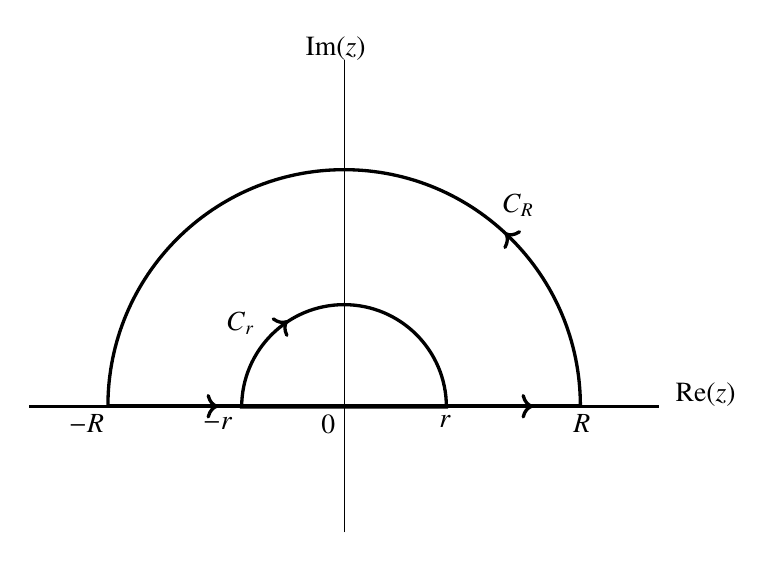
\begin{tikzpicture}
\draw (0,-1) -- (0,5); 
%\draw (-5,0.65) -- (5,0.65); 
\def\Radius{3}
  \path
    (-\Radius, 1) coordinate (A)
    -- coordinate (M)
    (\Radius, 0) coordinate (B)
    (M) +(60:\Radius) coordinate (C)
    +(2:\Radius) coordinate (D)
  ;
\draw[
      very thick,  decoration={markings, mark=at position -0.84 with {\arrow{>}}},
        postaction={decorate}
        ]  
(D) arc(0:180:\Radius) -- cycle;

\def\Radius{1.3}
  \path
    (-\Radius, 1) coordinate (A)
    -- coordinate (M)
    (\Radius, 0) coordinate (B)
    (M) +(60:\Radius) coordinate (C)
    +(4:\Radius) coordinate (D)
  ;

\draw[
      very thick,  decoration={markings, mark=at position 0.44 with {\arrow{<}}},
        postaction={decorate}
        ]  

 (D) arc(0:180:\Radius) -- cycle;
  
\begin{scope}[very thick,decoration={markings,mark=at position 0.8 with {\arrow{>}}}]
\begin{scope}[very thick,decoration={markings,mark=at position 0.3 with {\arrow{>}}}] 
\draw[postaction={decorate}] (-4,0.6)--(4,0.6);
\node[below right= 1mm of {(-0.7,5.5)}] {$\text{Im}(z)$};
\node[below right= 1mm of {(-3.7,0.7)}] {$-R$};
\node[below right= 1mm of {(-2,0.7)}] {$-r$};
\node[below right= 1mm of {(-0.5,0.7)}] {$0$};
\node[below right= 1mm of {(1,0.7)}] {$r$};
\node[below right= 1mm of {(2.7,0.7)}] {$R$};
\node[below right= 1mm of {(4,1.1)}] {$\text{Re}(z)$};
\node[below right= 1mm of {(1.8,3.5)}] {$C_{R}$};
\node[below right= 1mm of {(-1.7,2)}] {$C_{r}$};
\end{scope}
\end{scope}
\end{tikzpicture}
%\end{document}
}
\caption{}
\label{fig:origin_contour}
\end{figure}

%\begin{figure}[!h]
%\centering
%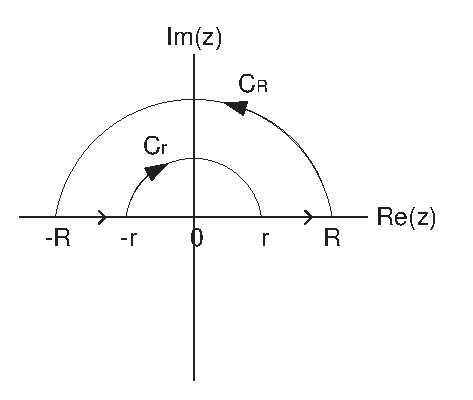
\includegraphics[width=\columnwidth]{./figs/origin_contour.ps}
%\caption{}
%\label{fig:origin_contour}
%\end{figure}
\begin{problem}
Using a suitable contour, evaluate $F(t), t > 0$.
\end{problem}
\begin{definition}
The residue of a function $f(z)$ at $z =c$ is defined as
\begin{equation}
\res{z=c}f(z) = \operatorname {Res} (f,c)={1 \over 2\pi i}\ointctrclockwise\limits _{\Gamma }f(z)\,dz
\end{equation}
where $c$ lies inside $\Gamma$.
\end{definition}
\begin{problem}
Find the inverse $Z$ transform of 
\begin{equation}
X(z) = \frac{1}{1-\frac{1}{2}z^{-1}}\quad \abs{z} > \frac{1}{2}
\end{equation}
\end{problem}
\begin{problem}
Find the inverse $Z$ transform of 
\begin{equation}
X(z) = \frac{1}{1-\frac{1}{2}z^{-1}}\quad \abs{z} < \frac{1}{2}
\end{equation}
\end{problem}
\begin{problem}
Let 
\begin{equation}
X\brak{z} = \frac{1-a^2}{\brak{1-az}\brak{1-az^{-1}}}, \quad \text{ROC}: a < \abs{z} < \frac{1}{a}, 
\end{equation}
$0 < a< 1$.  Determine $x(n)$
\end{problem}
\end{document}


